\documentclass[tikz,border=8pt]{standalone}
\usetikzlibrary{arrows.meta,decorations.pathmorphing}
\begin{document}
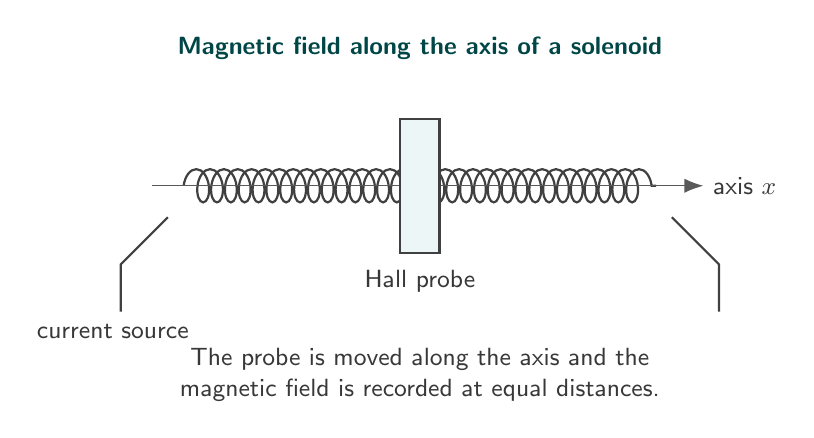
\begin{tikzpicture}[
  line/.style={draw=black!75,line width=0.8pt},
  label/.style={font=\sffamily\small,text=black!78},
  title/.style={font=\sffamily\bfseries\small,text=teal!55!black},
]
\node[title] at (0,3.15) {Magnetic field along the axis of a solenoid};
\draw[line,decorate,decoration={coil,aspect=0.55,segment length=5pt,amplitude=6pt}] (-3,1.4) -- (3,1.4);
\draw[-{Latex[length=2.4mm]},black!65] (-3.4,1.4) -- (3.6,1.4);
\node[label,right] at (3.6,1.4) {axis $x$};
\draw[line,fill=teal!7] (-0.25,0.55) rectangle (0.25,2.25);
\node[label,below] at (0,0.45) {Hall probe};
\draw[line] (-3.2,1.0) -- (-3.8,0.4) -- (-3.8,-0.2);
\draw[line] (3.2,1.0) -- (3.8,0.4) -- (3.8,-0.2);
\node[label] at (-3.9,-0.45) {current source};
\node[label,align=center,text width=8.4cm] at (0,-1.0)
  {The probe is moved along the axis and the magnetic field is recorded at equal distances.};
\end{tikzpicture}
\end{document}
